\subsection{CDCL}
\label{ss:cdcl}
All the methods to generate a backbone of a formula $F$ that are described in this thesis essentially rely on calculating various models of $F$, so it makes sense to describe a method to do that in depth. The current state-of-the-art algorithm to do this is the $Conflict\;Driven\;Clause\;Learning$ algorithm, or $CDCL$ for short. This algorithm was first published as $"GRASP"$ in \cite{GRASP}. An earlier algorithm for the SAT problem, which $CDCL$ is essentially based upon is the $DPLL$ algorithm \cite{dpll} published in 1962. However for this thesis I worked with the $CDCL$ implementation available in the $Sat4J$ library that is heavily based on $MiniSAT$ which can be read about in \cite{minisat}. Understanding of the employed SAT solver will become useful in later chapters, when I explain backbone computation strategies based on it.

\subsubsection{Storing solver state}

In this algorithm, a so-called $CDCL\;table$ is used as a special dataset to document how and why variables were assigned to either $\top$ or $\bot$. This table, which behaves like a stack, stores the succession of assignments with four values for each assignment.
\begin{itemize}
\item The affected variable.
\item The value that the variable was assigned to.
\item The reason for the assignment. This can be one of two cases, either $Unit$ or $Decision$.
\begin{itemize}
\item $Unit$ assignments happen, when a clause has all but one of its literals unsatisfied. Since all clauses have to be satisfied for a CNF formula to be satisfied, that last literal must be assigned a value that satisfies it and its clause. Entries in the CDCL table that refer to a unit assignment also store a reference to the clause that required the assignment. A clause that fulfills the above condition and requires an assignment can be called a $unit\; clause$ or that it $is\; unit$.
\item $Decisions$ happen when no clause is in the unit state. In theory, in this case you are free to pick any variable and assign it either $\top$ or $\bot$. 
\end{itemize}
\item The $level$ of the assignment. This level increases with each decision and starts at 0, where unit assignments before any decision are stored.
\end{itemize}

\subsubsection{Reducing search space}
The purpose of unit assignments is to reduce the amount of futile computational effort. The solving process for a formula can be modeled as the traversal of a search tree, where each node corresponds to an individual assignment and every leaf node to a complete assignment that might be satisfying or not\footnote
{
	Sadly the size of such a tree makes it impractical to actually implement SAT solving like this.
}. However, given that you can stop to search once a single clause is unsatisfied, you can disqualify many branches of the tree early, for example when the assignments in your tree path so far require some additional assignment for some clause, which would be a $unit\; clause$. Going the other way in the tree at that particular node will never result in a satisfying model.

The solver will now fill the table with assignments, unit assignments if possible or decisions otherwise, until one of two things happens. Either the formula becomes satisfied\footnote{
	In this case only an implicant is returned. If you want a complete model, you can keep making decisions until all variables are assigned and return the assignments after that. However once you have an implicant, you are free to assign the remaining variables to anything you want, as the formula is already satisfied and further assignments cannot change that.}
 in which case the assignments that are stored in the CDCL table are returned as a model.


\subsubsection{Learning from conflicts}
%cant put the figure higher, because it makes some weird layouting mess.
\begin{wrapfigure}{r}{8cm}
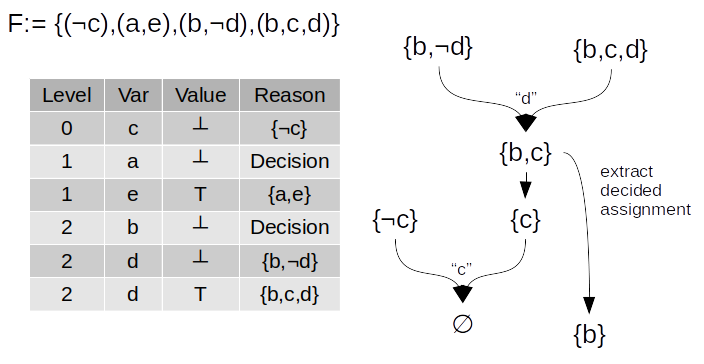
\includegraphics[width=8cm]{reso}
\caption{Example of a resolution. Shown is a formula, the content of the CDCL table at the point of conflict in variable $d$ and the resolution graph. The resulting learned clause is $\{b\}$.}
\label{fig:resolution}
\end{wrapfigure}

The other possibility is that you run into a contradiction. Here a unit clause requires that a variable is assigned a value $b$, but it is already assigned $\neg b$. If the assignments have a reason (a unit clause), then some of the variables in these clauses must be assigned differently (since they were unit then), so we can connect the reasons for our conflict to other assignments. Repeating this we sometimes meet decisions instead of unit clauses as reason. Collecting these decisions, we end with the precise combination of assignment decisions that resulted in the conflict. 


This process of following assignments through their reasons is called $resolution$ and can be briefly explained with the following formula:
$$
r_\lambda(c_1,c_2) = (c_1 \textbackslash \{\lambda\}) \cup (c_2 \textbackslash \{\neg \lambda\})
$$
The resolvent $r$ consists of all literals of the two clauses that are resolved, where in this case $c_1$ contains $\lambda$ and $c_2$ contains $\neg \lambda$. This precondition is given in this case, because $c_1$ is the reason for the assignment of $\lambda$ to $\top$ and $c_2$ the reason for assigning $\lambda$ to $\bot$. 

Figure \ref{fig:resolution} shows this with an example, where a conflict in variable $d$ happened. First the clauses $\{b,\neg d\}$ and $\{c,b,d\}$ are resolved over the variable $d$. Then $b$ is extracted for the learned clause, as its reason was a decision and not a unit clause. Finally $\{c\}$ and $\{\neg c\}$ are resolved over $c$, resulting in the empty set. The learned clause is $\{b\}$.\\
An alternative resolution scheme would leave literals that stem from decisions in the working set until the end, but here they are extracted on first extraction. Otherwise, these literals would be inspected multiple times.


Once collected, this set of decisions must be taken back, by reversing the assignments up until the first of these decisions, as this path through the search tree results in a conflict and will not end in models. 

We also add the clause to our formula as a $learned\; clause$. This clause serves to prevent the particular combination of assignments that led to our conflict. The resulting formula will still be completely equivalent to before. It merely stores the information that we gained through analysis of our conflict to prevent it from happening again.

However it is also possible that we end up with reasons for assignments that do not end in a decision. This would mean that all reasons were axiomatic assignments, for example when a formula contains a clause with only a single literal in it\footnote{A simple example: A formula contains the two clauses $\{a\}$ and $\{\neg a\}$. Resolving these two results in the empty set.}  .
In this case the formula implies a contradiction and the clause that we would learn from this would be empty, unsatisfiable.


\begin{algorithm}
\DontPrintSemicolon
\KwIn{A formula $F$ in CNF}
\KwOut{A CDCL table which implies an implicant for $F$, or $\perp$ if $F$ is not satisfiable}
$level \gets 0$\;
$table \gets emptyList$\;
\While{$1$}{
	$table.pushAll(F.getUnits())$\;
	\If{$\exists\;conflicting\; assignment$}{
		\If{$level = 0$}{\Return{$ \perp$}}
		\Else{$level \gets backtrackAndLearn(F,table)$}
	}\ElseIf{$F\;is\;fulfilled$}{
		\Return{$table$}
	}\Else{
		$level++$\;
		$l \gets any\;free\;variable$\;
		$l.assign(either\; \top\; or\; \bot)$\;
		$table.pushDecision(l)$\;
	}
}
\caption{{\sc CDCL algorithm}}
\end{algorithm}

\subsubsection{Decision heuristics}

Concerning the decisions, depending on the particular formula, it is possible that some assignments make it easier to solve the formula than others and some decisions might lead to a completely unsatisfied clause. To prevent this, there exists a range of heuristics that try to pick a variable and corresponding assignment that would lead to a satisfying model without complications. A typical one would be to measure the activity of a variable, which is an estimate of how often it was involved in conflicts. The heuristic would then always pick the variable with the lowest activity, since it would most likely be unproblematic to assign one or the other value to it. To choose the boolean value that should be assigned to it, a good strategy can be to remember the value that each variable was assigned to on the last occasion and this time give it the opposite one. When a variables assignment is removed through conflict resolution, going in the complete opposite direction with the assignments has a good chance to work out better.

%For this you would typically measure how often the variable was involved in conflicts and prefer not to decide on such difficult variables but . It is assumed that difficult formulas are so because of individual difficult variables. If you decide on these early, you have a 50-50 chance that you either found the correct assignment or at least learned a useful clause from a conflict.

\subsubsection{Notation in algorithms}

As is usually done in literature, calls to SAT solvers such as CDCL in code listings are written as $(outc,\nu) = SAT(F)$. Here, two values are returned. $outc$ is a boolean value that simply states whether $F$ turned out to be satisfiable or not, the result of which is often written as $SAT$ and $UNSAT$. Only if $outc$ equals to $SAT$, the second return parameter $\nu$ can have a meaningful value, which would be the model that was found and satisfies $F$. In some of the algorithms listed in this thesis, one of the return parameters is not used at all. In that case I write $(\_,\nu) = SAT(F)$ or $(outc,\_) = SAT(F)$ to indicate that either $outc$ or $\nu$ is discarded.

